\section{频散与波场偏移精确度}
\label{sec:4.3}

频散系由不同频率成分以不同速度传播而形成。虽然许多读者可能听到过冰在冻结的湖
面和河面上滑动时的声音,可是在日常生活中却很少听说到频散物理现象。正在破裂的冰所
引起的弹性波,它的传播就具有频散性质,使得破裂声变成敲击震动的调子。地震波沿地表
面传播时一般可观察到波散,但对内部发生的反射波则简直很难察觉到有波散现象。在地震
数据处理中,频散是一种讨厌的事,对于处理的设计者来说,频散现象是严重的妨害和困
扰。频散现象主要由有限差分方法形成,因为微分算子和差分算子在高频上并不一致.进行
更加密的采样总可以压制掉频散,检查是否这样作了,正是生产分析人员的任务。图\ref{fig:dspr/freqdisp}
所示是某些经过频散的脉冲。

\begin{figure}[H]
\centering
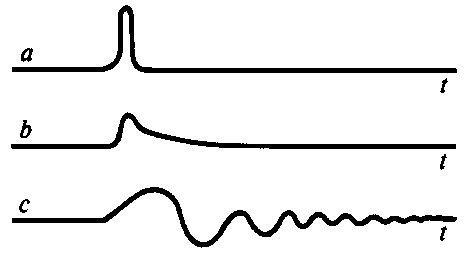
\includegraphics[width=0.65\textwidth]{dspr/freqdisp}
\caption[freqdisp]{(a)脉冲。(b)稍微频散的脉冲,因高频耗散而形成。
(c)具有显著频散的脉冲,这类频散可以因数据处理不小心而形成}
\label{fig:dspr/freqdisp}
\end{figure}

由数据处理所引起的频散可以是关于数据正处于发
生假频的危险之中的一种很有用的警告。各种频率域方
法均不依靠差分算子,所以它们都有不会表现出频散现
象的好处,不过这种好处也有附带的后果,即(1)没
有频散只限于恒定盼物质性质和(2)没有关于频散的
警告迹象就出现了空间假频。

图\ref{fig:dspr/taner}是偏移资料中出现频散的例子,上图为共
深度点叠加剖面。中间的图是处理之后的剖面,处理时
尚未企图控制频散现象,200号炮点附近在4秒时间上存
在有严重的频散现象。下面的图则是经过重新处理之后
的剖面,频散现象已大大减弱。

\begin{figure}[H]
\centering
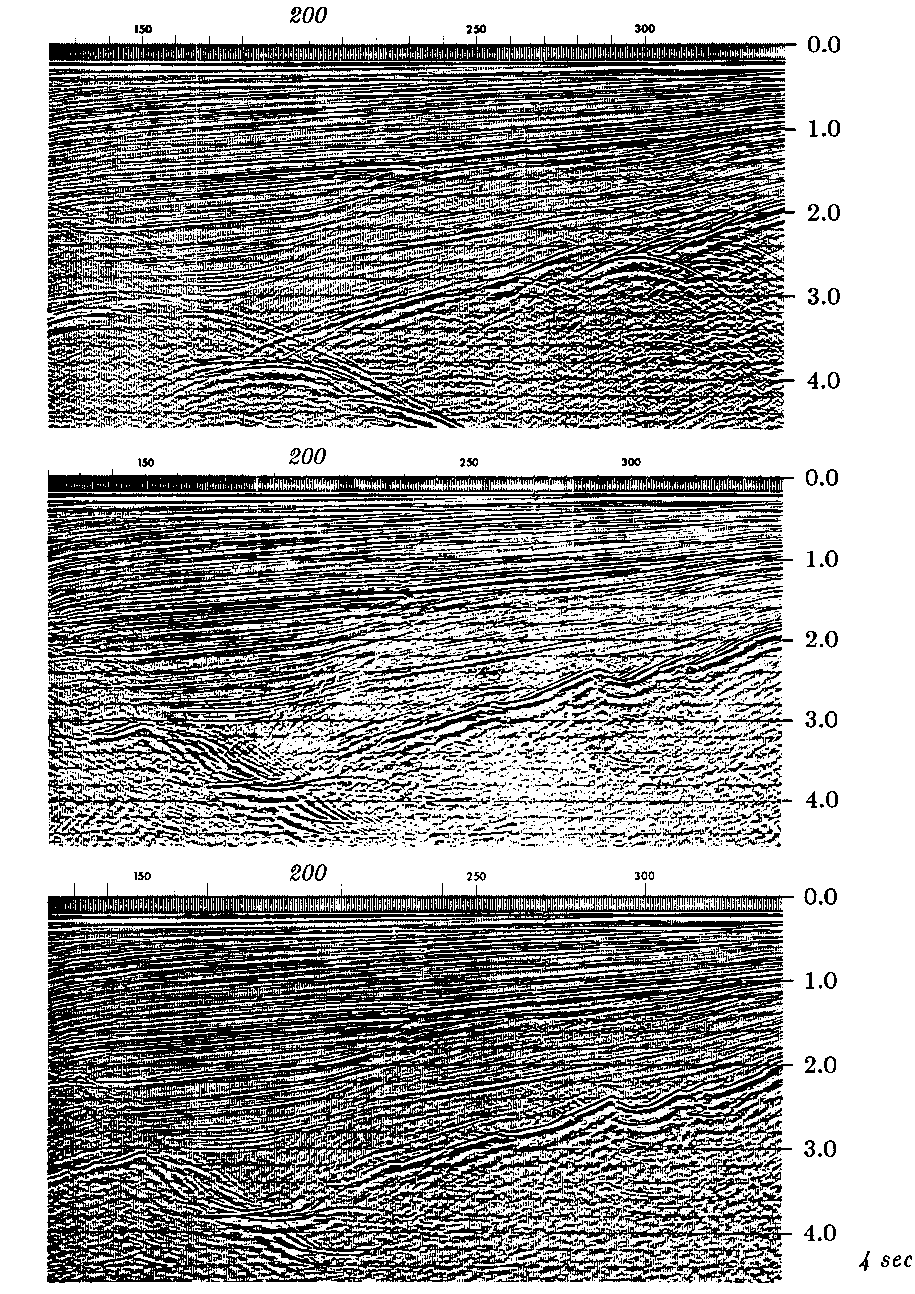
\includegraphics[width=0.65\textwidth]{dspr/taner}
\caption[taner]{克服和控制频散现象(据Taner与Koehler)}
\label{fig:dspr/taner}
\end{figure}

% \subsection{不垂直于波阵面的射线}
% \label{sec:4.2.1}

% 各向异性的意思是指,沿不同方向传播的波各以不同速度传播。各向异性并不意味着速
% 度是空间位置的函数,因而各向异性并不引起射线弯曲。有关各向异性的独有现象是,射线
% 不垂直于波阵面,可用图\ref{fig:dspr/aniso}说明这种思想。该图的左图表示由位于原点的点震源发射出
% 的球形波阵面,这就是通常说的各向同性情形。右图表示15°偏移方程的非球形波阵面,注
% 意,它们在接近$z$轴处是近乎球形波阵面的,但是远离该轴时,它们同中心位于原点的球形
% 就差得远了。



% 惠更斯二次震源所形成的理想波阵面应是一个半圆。由15°外推方程形成的二次震源波
% 阵面应是椭圆;由45°外推方程形成的二次震源波阵面是一种有趣的心脏形,这些均绘于图
% 图\ref{fig:dspr/anisoxz}
% 内。实际上,棉圆与心脏形之顶部很少能被看
% 到,因为它们均位于指数衰减区域之内,而且沿欠轴
% 的点距极少可能加密到足以显示它们所需的低于空间假
% 频的程度。采用45°外推程序时,有时能在$(x,t)$平
% 面内看出该心脏形曲线的中心,图\ref{fig:dspr/anisoxt}中所绘直线即
% 用以表示该中心。采闱45°绕射程序处理时的情形如图\ref{fig:dspr/45imp}所示。

% \begin{figure}[H]
% \centering
% 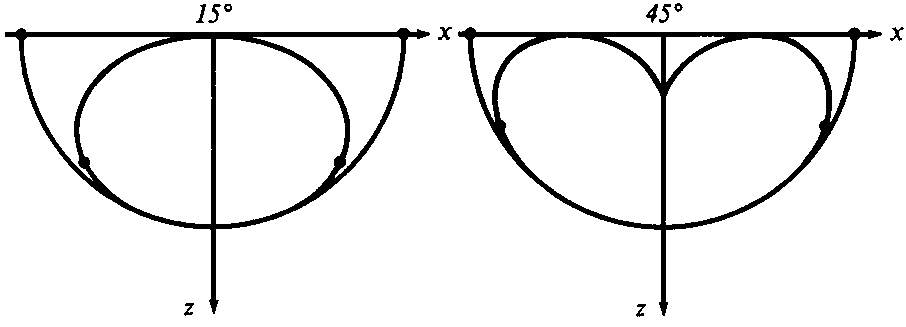
\includegraphics[width=0.65\textwidth]{dspr/anisoxz}
% \caption[anisoxz]{15°外推方程的波阵面(左图)及45°外推方程的波阵面(右图),二者均内接于半圆之内。
% 凡属$\frac{vk_x}{\omega}=\sin\theta=\pm1$的波均以小黑点表示,倏逝波均在曲线脱离半圆之处的小圆点
% 以上(据Rothman)}
% \label{fig:dspr/anisoxz}
% \end{figure}

% \begin{figure}[H]
% \centering
% 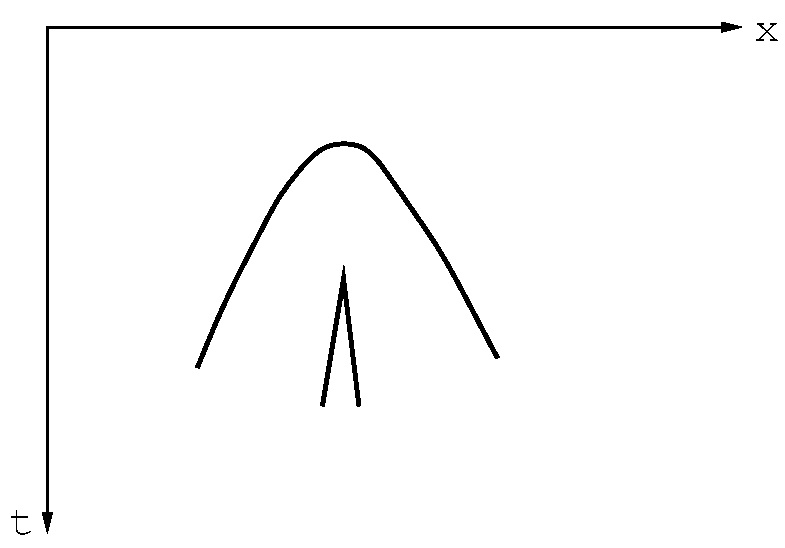
\includegraphics[width=0.65\textwidth]{dspr/anisoxt}
% \caption[anisoxt]{45°外推方程的心脏形理论曲线。尖点
% 出现在指数衰减区域内(据Rothman)}
% \label{fig:dspr/anisoxt}
% \end{figure}

% \subsection{波阵面方向与能量速度}
% \label{sec:4.2.2}

% 在普通的波动传播理论中,能量传播方向是垂直于
% 波阵面的。当存在有各向异性弥散时,角度将不再是呈直角了。

% \begin{figure}[H]
% \centering
% 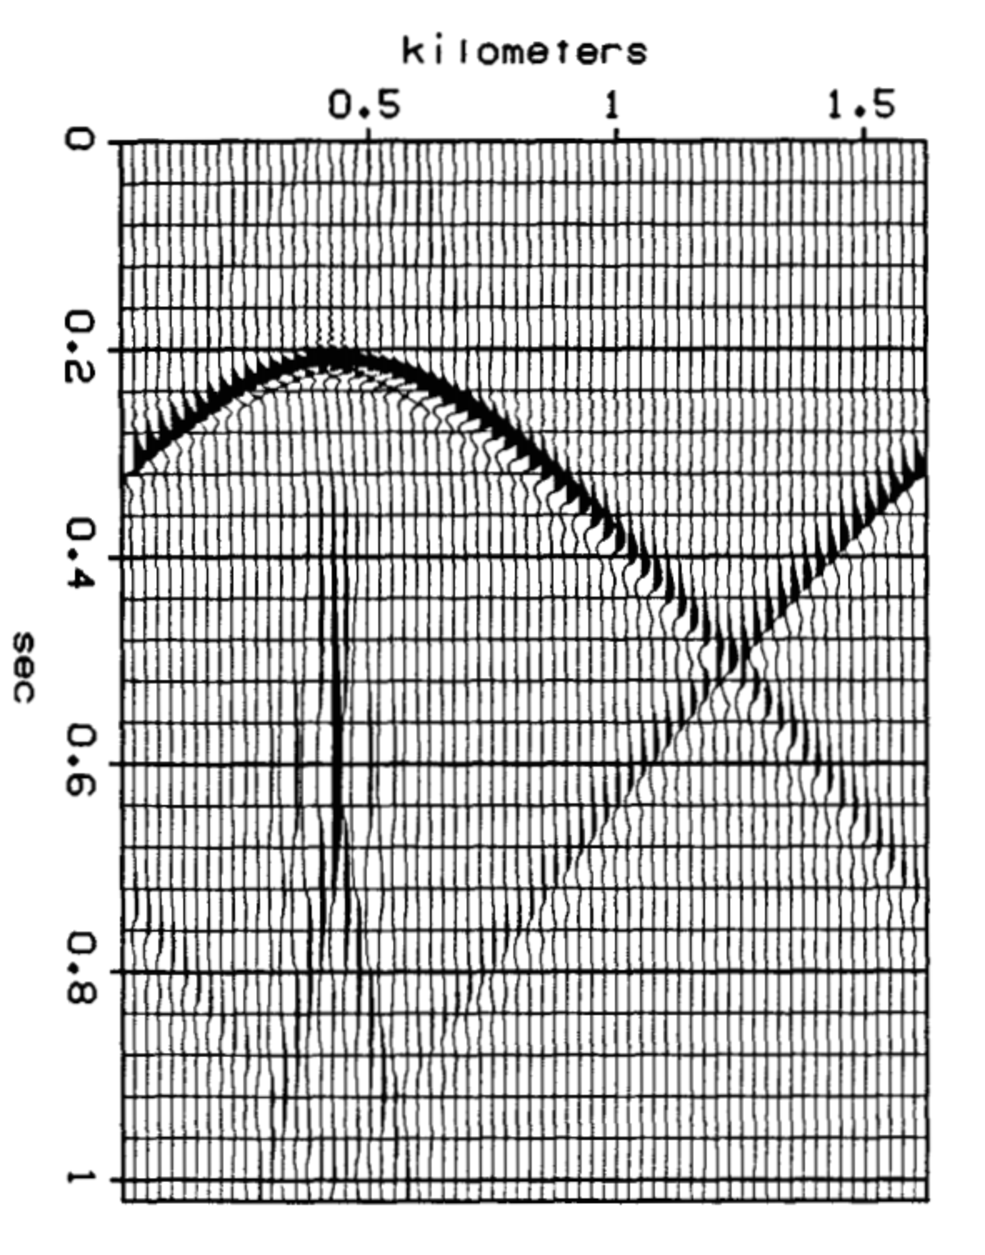
\includegraphics[width=0.65\textwidth]{dspr/45imp}
% \caption[45imp]{45°波场外推方程的脉冲响应。$t_0$时间
% 以前的初至是折叠频率产生的影响。}
% \label{fig:dspr/45imp}
% \end{figure}

% 沿地表能看到的水平视速度为$dx/dt$,沿垂直方向
% 的视速度(如在井中所见)为$dz/dt$,根据几何关系可
% 知,这些视速度全都大于波动传播速度。大小与速度呈
% 反比而方向垂直于波阵面的一个向量,称作慢度向量
% \begin{equation*}
% \text{慢度向量}=(\frac{dt}{dx},\frac{dt}{dz})
% \end{equation*}
% 沿慢度向量的方向行进但具有波阵面法线速度的一种向
% 量,定义为相速度向量,更精确地说,相速度向量等于慢度向量除以其平方幅度
% \begin{equation*}
% \text{相速度}=\frac{(\frac{dt}{dx},\frac{dt}{dz})}{(\frac{dt}{dx})^2+(\frac{dt}{dz})^2}
% \end{equation*}

% 就正弦形扰动$\exp(i\phi)=\exp(-i\omega t+ik_xx+ik_zz)$
% 而言,可令相位$\phi$等于常数
% \begin{equation*}
% d\phi=-\omega dt+k_xdx+k_zdz=0
% \end{equation*}
% 因而,在Fourier空间内,慢度向量为
% \begin{subequations}
% \begin{equation}
% \text{慢度向量}=(\frac{k_x}{\omega},\frac{k_z}{\omega})
% \label{eq:ex4.2.1a}
% \end{equation}
% 要导出能量传播方向则更为困难一点,不过可由所谓群速度向量导出它
% \begin{equation}
% \text{群速度向量}=(\frac{\partial}{\k_x},\frac{\partial }{k_z})\omega(k_x,k_z)
% \label{eq:ex4.2.1b}
% \end{equation}
% \end{subequations}
% 对于标量波动方程应有$\omega^2/v^2=k_x^2+k_z^2$,由是迸行微分并代入,可以证明群速度向量原来同
% 相速度向量是相同的。最熟悉的弥散类型是频散,这时不同频率是以不同速度传播。以后本
% 节将会指出,熟悉的外推方程(15°的,45°的等等)并不表现出频散性质。那就是说,作为
% $\omega$与角度$k_x/\omega$的函数,在这些方程中的速度并不依赖于频率$\omega$。换句话说,图\ref{fig:dspr/anisoxz}中的椭圆形与心脏形曲线均与频率无关。

% 各向异性弥散的一个有趣现象是,能量看起来好像是沿某一个方向在行进着而其实它实
% 际上是在沿另一个方向行进着。当群速度有一个向下分量而相速度有一向上分量时,就会出现
% 这种现象。描述45°外推方程之弥散关系的图\ref{fig:dspr/group15}就是一个例子,从原点至弥散曲线所画之
% 箭头表示沿波阵面法线方向的慢度向量,注意到群速度以式\ref{eq:ex4.2.1b}中的梯度算子来每
% 义,现在就能用图解方法确定相应的群速度方向。试将$\omega$值考虑为一个小山的高度,$k_z$就是
% 从该$\omega$山头指向南而$k_x$则指向东,于是,弥散关系曲线就是等高线,按不同的比例标度绘出图
% \ref{fig:dspr/group15}就形成了不同频率的数值,沿梯度方向的群速度则是垂直于各$\omega$的等值线。

% 采用活动电影形式可以非常清楚地识别出各向异性弥散现象,尽管在如图\ref{fig:dspr/prism}所示的
% 单个画面上也可以认识出来。图\ref{fig:dspr/prism}中所绘直线是解释能量由顶部进入,经过棱镜,在棱
% 镜的45°淘度一侧反射,再从画面的一侧反射,最后进入图中某一个区域,该区域有足够的
% 大小,因而许多波阵面不致群集一起,足以识别出能量看似向上传播其实真正的是向下传
% 播。

% \begin{figure}[H]
% \centering
% 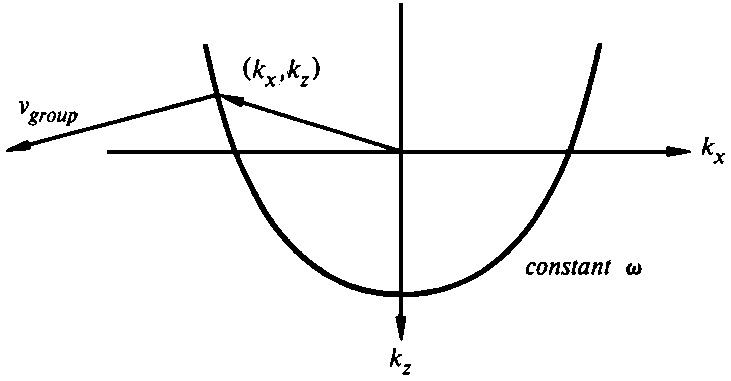
\includegraphics[width=0.65\textwidth]{dspr/group15}
% \caption[group15]{表示群速度向量与慢度向量的向下外推方程弥散关系曲线(据Rothman)}
% \label{fig:dspr/group15}
% \end{figure}

% \begin{figure}[H]
% \centering
% 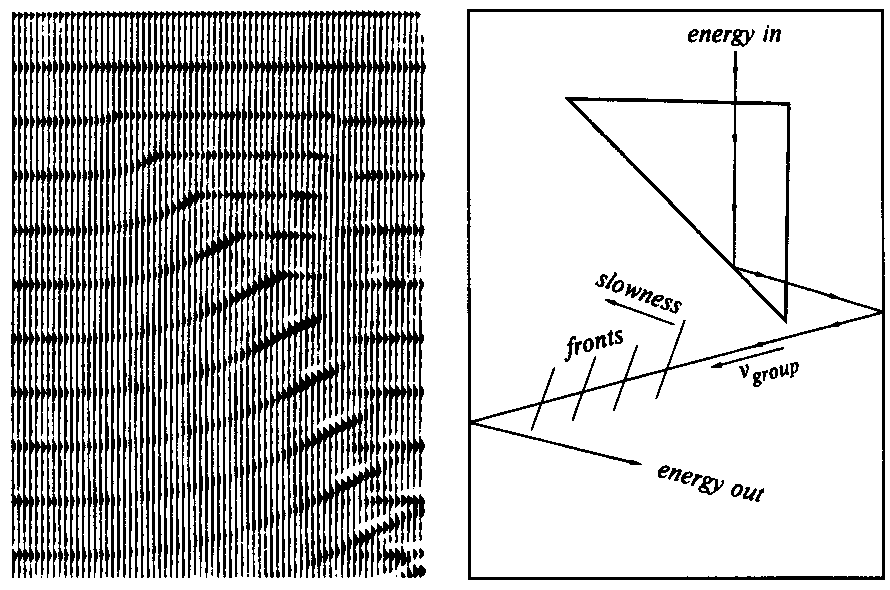
\includegraphics[width=0.65\textwidth]{dspr/prism}
% \caption[prism]{四种不同频率的平面波,传播通过一个具有$45$°角度的棱镜。左图为
% 波场,右图是说明能量的不同方向和波阵面法线方向的射线解释图(据Estevez)}
% \label{fig:dspr/prism}
% \end{figure}

% 当你考虑到计算波场所用的程序时,
% 在图\ref{fig:dspr/prism}中无论能量还是信息都不可能
% 向上传播,这一点就应更清楚了。程序并
% 没把整个画面都输入于内存,它每次紧挨着前一个条带,一次计算出一个水平条
% 带。所以活动电影中的波阵面是貌似向上
% 移动,似乎很难令人理解。从理论上说,利用45°方程的波场外推方法是不能指望
% 可以处理达到90°的角度的,而图\ref{fig:dspr/prism}中
% 的例子却尚表明,虽然是以一种有点不正
% 常的方式、但确实是可以处理这些极端情形的。

% 有一次,我在地质上属于是逆掩断层地区的反射地震剖面上观察到过类似的环境条件,
% 这个剖面目前已不能为我所用,现在大概早就从拥有者的底片中消失了,所以我仅能根据记
% 忆提供如图\ref{fig:dspr/overthrust}所示的简图。图中,速度随深度而增大,引起射线向上弯曲,并从逆掩断
% 层的下侧反射。为了想知道在波动方程中究竟正在发生什么事,画出如图\ref{fig:dspr/disper2z}所示的两种不同速度时的弥散曲线,将是很有帮助的。

% \begin{figure}[H]
% \centering
% 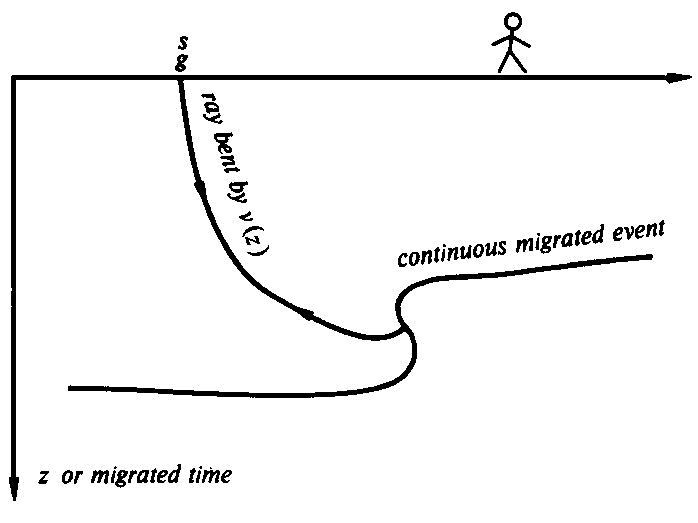
\includegraphics[width=0.65\textwidth]{dspr/overthrust}
% \caption[overthrust]{从逆掩断层下侧发生反射的射线}
% \label{fig:dspr/overthrust}
% \end{figure}

% \begin{figure}[H]
% \centering
% 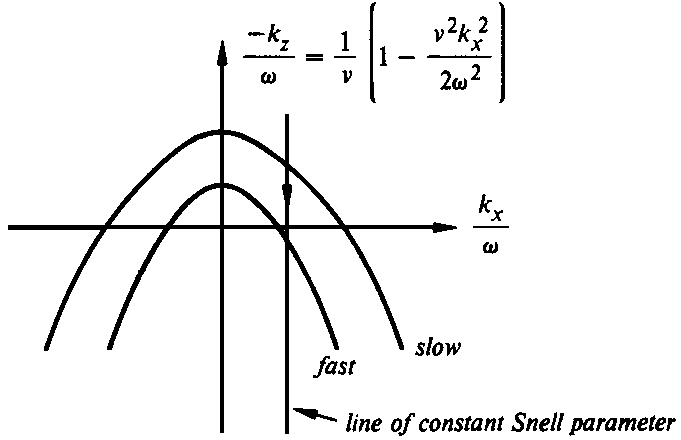
\includegraphics[width=0.65\textwidth]{dspr/disper2z}
% \caption[disper2z]{两种不同速度$v_{fast}$与$v_{slow}$时的弥散曲线}
% \label{fig:dspr/disper2z}
% \end{figure}

% 具有某种特定时差心的一小部分能量在近地表处(即这时适用低速弥散曲
% 线)以某种普通的角度开始向下延拓,但是当遇到较深层具有高速的地层时,这时应适用高
% 速弥散曲线,在此情形下由图\ref{fig:dspr/disper2z}可知,相同的时差$k_x/\omega$却预示着应有负值的相速度。虽
% 然上冲角的大小未必正确,可总的图象大体是合适的,它很像图\ref{fig:dspr/prism}中所示的情形。如果你想要定量上是正确的偏移,可参阅\ref{sec:4.5}节,或者想要有点完全不同的偏移,则可参阅
% Kosloff等(1983)和Baysal等(1983)提出的方法。

% \subsection{偏移误差分析}
% \label{sec:4.2.3}

% 利用相速度概念可以对平坦规则的倾斜反射面作整钵分析,仅在同时存在有一个以上的
% 传播角度时,才需要利用群速度概念。采用点源散射体响应时,会出现这种同时性的要求,
% 在沿倾斜地层存在有可变反射振幅时,也会出现这种要求。群速度之所以需要,是因为表示
% 弯曲同相轴或振幅异常,要求平面波传播角度有一定范围。与此类似,在时间序列分析中,
% 一个经过振輻调制的正弦波之Fourier变换需要有一定频带范围内的正弦谐波。

% 图\ref{fig:dspr/undermig}所示是光滑平坦倾斜地层,因为用某种有理平方根近似或某种数值近似所定义
% 的波数$\hat{k_z}$同$k_z$的正确平方根值并不符合一致,以致偏移不足。

% \begin{figure}[H]
% \centering
% 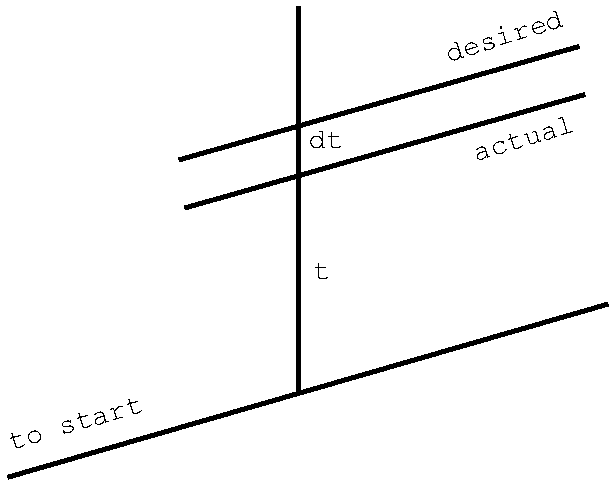
\includegraphics[width=0.65\textwidth]{dspr/undermig}
% \caption[undermig]{偏移不足的倾斜反射面}
% \label{fig:dspr/undermig}
% \end{figure}

% 图\ref{fig:dspr/undermig}中的误差全部是某种时移误差。由于沿反射面的反射系数为常数,识别不出什
% 么横向位移误差。该时间误差在理论上可按下式确定:
% \begin{equation}
% \frac{dt}{t}\approx\frac{dz}{z}\approx\frac{\hat{k_z}-k_z}{k_z}
% \label{eq.ex4.2.2}
% \end{equation}
% 就所谓15°外推方程来说,在25°度时所造成的相位误差可证明大约为百分之五十。

% 其次,我们要确定一下双曲线收缩压扁时的误差。图\ref{fig:dspr/errcollapse}所示是一个双曲线的向下延
% 拓,为清晰起见,向下延拓没有沿指向聚焦点的所有路径进行。选定某个斜率$p$就可选出具
% 有某个Snell参量$p=dt/dx$的射线。试想像有一斜率为$p$的切线段切于各双曲线。如果斜率
% 为p之处有一点振幅异常。那末,你就能在各个双曲面上追踪出它。

% \begin{figure}[H]
% \centering
% 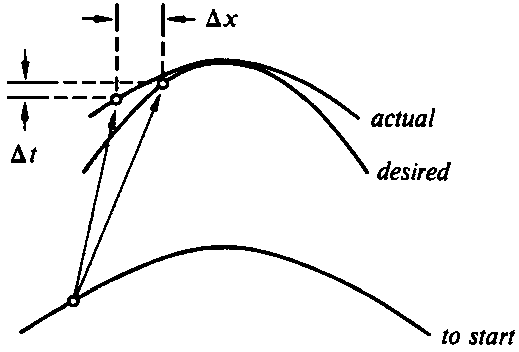
\includegraphics[width=0.65\textwidth]{dspr/errcollapse}
% \caption[errcollapse]{双曲线挤缩收敛误差。
% 注意,实际曲线位于所期望曲线之上,但是
% 实际的点却是位于所期望点之下}
% \label{fig:dspr/errcollapse}
% \end{figure}

% 在图\ref{fig:dspr/errcollapse}中,时间移动量太小了,横向移动距离同样也很小。实际上,具有$r_0=1$的
% 15°方程的误差,有时采取把深度坐标$z$或者速度$v$增大6\%的办法就能被补偿掉。各误差量可
% 根据下式计算
% \begin{subequations}
% \begin{equation}
% \frac{\Delta t}{t}=\frac{\frac{\partial}{\partial \omega}(\hat{k_z}-k_z)}{\frac{\partial}{\partial \omega}k_z}
% \label{eq:ex4.2.3a}
% \end{equation}
% \begin{equation}
% \frac{\Delta x}{x}=\frac{\frac{\partial}{\partial k_x}(\hat{k_z}-k_z)}{\frac{\partial}{\partial k_x}k_z}
% \label{eq:ex4.2.3b}
% \end{equation}
% \label{eq:ex4.2.3}
% \end{subequations}
% 式中,$k_z$取为$\omega$和$k_x$的函数。它证明,就15°外推方程而言,在角度为20°度时出现百分之五
% 十左右的群速度误差,因而群速度误差一般是要比相速度误差更为严重的。

% \subsection{群速度方程的导出}
% \label{sec:4.2.4}
% 在$(x,z)$空间的原点上之脉冲函数是许多Fourier分量的叠加结果:
% \begin{equation}
% \iint e^{+ik_xx+ik_zz}dk_xdk_z
% \label{eq:ex4.2.4}
% \end{equation}
% 根据物理规律(或许还有根据数值分析)所导出的弥散关系是$\omega$、$k_x$与$k_z$之间的一种函数关
% 系,比方说,以$\omega(k_x,k_z)$表示这种关系。由标量波动方程得出的就是这
% 一类弥散关系的最普通的例子。该方程的解为
% \begin{equation}
% e^{-i\omega t+ k_xx+ik_zz}
% \label{eq:ex4.2.5}
% \end{equation}
% 遍及$(k_x,k_z)$对式\ref{eq:ex4.2.5}进行积分,得出一种单频时间函数,该函数在$t=0$时就是
% 位于$(x,z)=(0,0)$点上的脉冲。在某个非常大的时间$t$时,这种函数的表达式为
% \begin{equation}
% \iint e^{-it[\omega(k_x,k_z)-k_xx/t-k_zz/t]}dk_xdk_z
% \label{eq:ex4.2.6}
% \end{equation}
% 在$t$非常之大时,被积函数是具有单位幅度的非常快速振荡之函数。因此,除非知道方括号
% 内的量在$(k_x,k_z)$空间相当广大的区域内近乎与$k_x$和$k_z$独立无关,否则这个积分将接近于
% 零。像求出一个二维函数之极大值和极小值的作法一样,就是说,采用令其各个偏导数等于
% 零的办法,就可以求出这样一种平点(flat spot)。这种分析方法即是众所围知的稳相法
% (stationary phase method)。由它得出
% \begin{subequations}
% \begin{equation}
% \frac{\partial}{\partial k_x}[]=\frac{\partial\omega}{\partial k_x}-\frac{x}{t}=0
% \label{eq:ex4.2.7a}
% \end{equation}
% \begin{equation}
% \frac{\partial}{\partial k_z}[]=\frac{\partial\omega}{\partial k_z}-\frac{z}{t}=0
% \label{eq:ex4.2.7b}
% \end{equation}
% \label{eq:ex4.2.7}
% \end{subequations}
% 所以,最终得出结论,在时间$t$时, 该扰动将位于
% \begin{equation}
% (x,z)=t(\frac{\partial\omega}{\partial k_x},\frac{\partial\omega}{\partial k_z})
% \label{eq:ex4.2.8}
% \end{equation}
% 由此证明群速度的定义是正确的。
% 现在让我们看一看图\ref{fig:dspr/anisoxz}中的15°外推方程情形下的波阵面是如何计算出来的。解出
% 15°弥散关系的$\omega$值并代入式\ref{eq:ex4.2.8},所得结果$(x,z)$证明是的一个函数,利用一
% 切可能的值就可绘出该图中的曲线。

% \subsection{能量偏移方程的导出}
% \label{sec:4.2.5}

% 现在以类似于导出群速度的方式来分析$(x,t)$空间内的能量偏移。将积分
% \begin{equation}
% \iint e^{iz[k_z(\omega,k_x)-\omega t/z+k_xx/2]}d\omega dk_x
% \label{eq:ex4.2.9}
% \end{equation}
% 内的深度z取得很大,结果就使能量趋向下列位置
% \begin{equation}
% (x,t)=z(-\frac{\partial k_z}{\partial k_x},\frac{\partial k_z}{\partial \omega})
% \label{eq:ex4.2.10}
% \end{equation}
% 这就证明了我们以前断言可以用式\ref{eq:ex4.2.3}来分析能量传播误差一事是正确的。式
% \ref{eq:ex4.2.10}也可用于计算图\ref{fig:dspr/anisoxt}中的曲线。稳相概念的有效性已为图
% \ref{fig:dspr/45imp}所证实,该图就是利
% 用反Fourier变换方法得到的。
% %
% \subsection{外推方程不具有频散性质}
% \label{sec:4.2.6}

% 为证明所熟悉的15°、45°等等的波场外推方法不是频散的,回想一下\ref{sec:2.2}节,在该节
% 中,弥散关系都具有$k_z/\omega=f(k_x/\omega)$
% 的形式,其中,$f$是某种半圆近似,比方说,15°近似
% 或45°近似。这种形式的弥散关系没有一种能够是频散的。作出式(4.2.10)所要求的求导运
% 算,你就会明白,虽然波阵面的$(x,t)$坐标通过Snell参量$vk_x/\omega$而与倾角有关,可它们并非明
% 显迪直接依赖于频率$\omega$。所以,实践中所观察到的任何频散并不是由15°或45°近似所产生的。
